\section{Hagan Rowlenstino A. S(1174040)}
\subsection{Menggunakan LeafletJS dengan MapProxy}
\begin{enumerate}
    \item Kita run terlebih dahulu MapProxy yang telah dibuat kemarin
    \hfill\break
    \begin{figure}[H]
		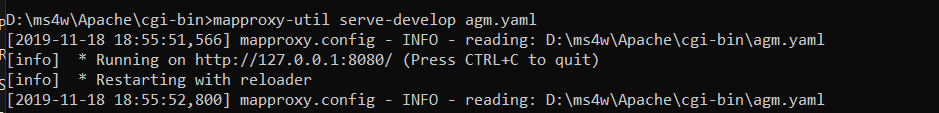
\includegraphics[width=12cm]{figures/1174040/Python4/1.PNG}
		\centering
		\caption{Gambar 1}
	\end{figure}
    \item Buka file contoh penggunaan LeafletJS yaitu basic.html di dalam folder leafletjs di dalam folder gede yang telah dibuat oleh Bpk.Rolly
    \hfill\break
    \begin{figure}[H]
		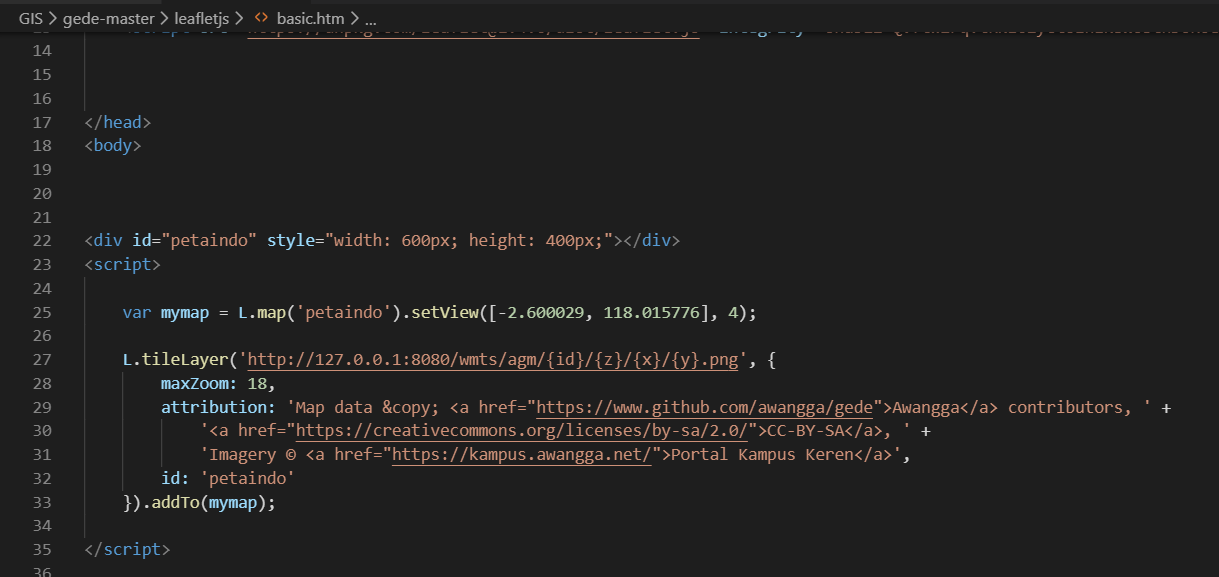
\includegraphics[width=12cm]{figures/1174040/Python4/2.PNG}
		\centering
		\caption{Gambar 2}
	\end{figure}
    \item Lalu buka file tersebut di browser, maka hasilnya akan seperti ini
    \hfill\break
    \begin{figure}[H]
		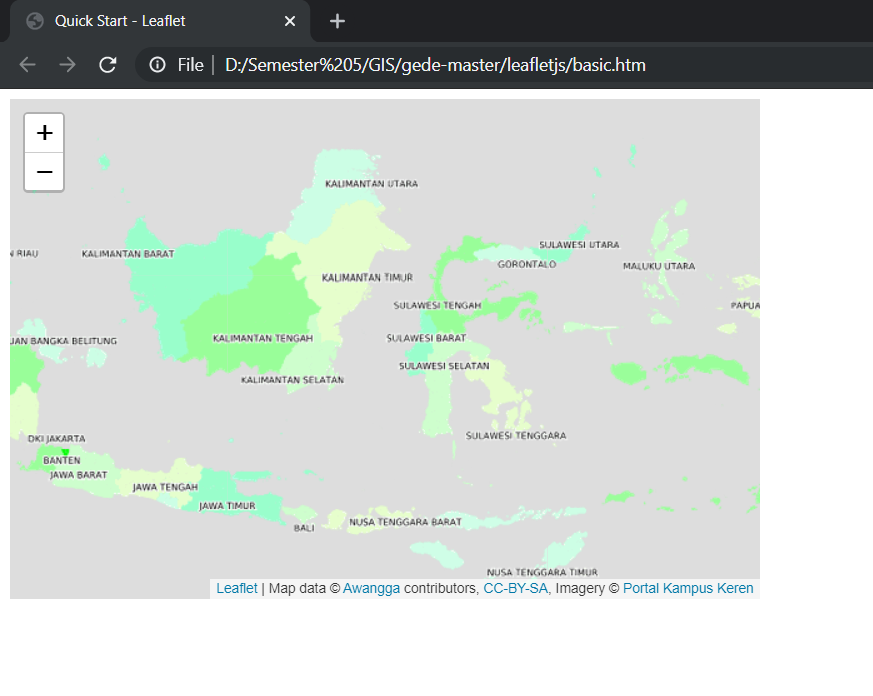
\includegraphics[width=12cm]{figures/1174040/Python4/3.PNG}
		\centering
		\caption{Gambar 3}
	\end{figure}
    \item Dengan leafletjs kita juga dapat menambahkan marker,circle, ataupun polygon dengan cara menggunakan seperti di gambar, contoh ini diambil
          dari file contoh kedua yaitu marker.html dari folder gede 
    \hfill\break
    \begin{figure}[H]
		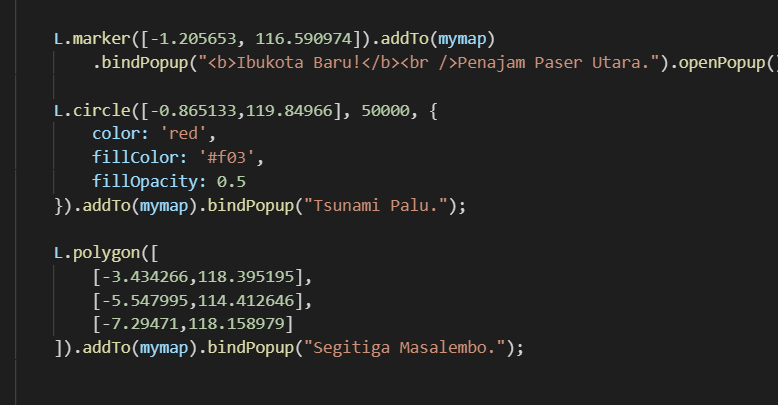
\includegraphics[width=12cm]{figures/1174040/Python4/4.PNG}
		\centering
		\caption{Gambar 4}
	\end{figure}
    \item Lalu buka file tersebut dengan browser dan hasilnya akan seperti pada di gambar
    \hfill\break
    \begin{figure}[H]
		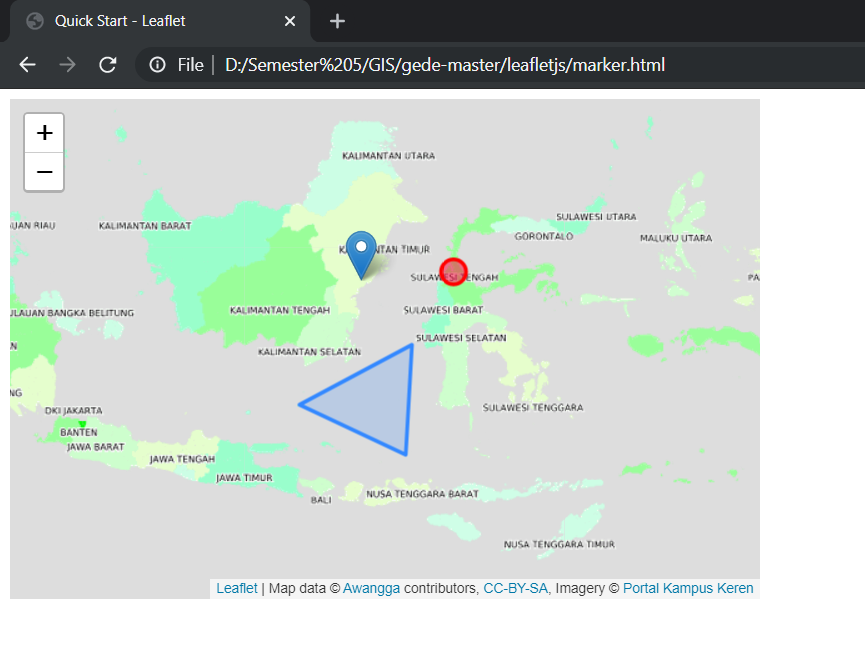
\includegraphics[width=12cm]{figures/1174040/Python4/5.PNG}
		\centering
		\caption{Gambar 5}
	\end{figure}
\end{enumerate}
\subsection{Link Youtube}
\href{https://www.youtube.com/watch?v=z3GK-cLmQT4}{Yotube Hagan}